\documentclass{beamer}
\usepackage{graphics}
\usepackage{epsfig}
\setbeamertemplate{navigation symbols}{}
\newcommand{\RR}{\ensuremath{\mathbb{R}}}
\newcommand{\NN}{\ensuremath{\mathbb{N}}}
\newcommand{\QQ}{\ensuremath{\mathbb{Q}}}
\newcommand{\CC}{\ensuremath{\mathbb{C}}}
\newcommand{\ZZ}{\ensuremath{\mathbb{Z}}}
\newcommand{\TT}{\ensuremath{\mathbb{T}}}
\newcommand{\HH}{\ensuremath{\mathbb{H}}}
\DeclareMathOperator{\Min}{Min}
\DeclareMathOperator{\Dom}{Dom}
\DeclareMathOperator{\vol}{vol}
\DeclareMathOperator{\Aut}{Aut}
\DeclareMathOperator{\Stab}{Stab}
\DeclareMathOperator{\Sym}{Sym}
\DeclareMathOperator{\Grp}{Grp}
\DeclareMathOperator{\Ker}{Ker}
\DeclareMathOperator{\GL}{GL}
\DeclareMathOperator{\SL}{SL}
\DeclareMathOperator{\Id}{Id}
\DeclareMathOperator{\mint}{min}
\DeclareMathOperator{\vertt}{vert}
\DeclareMathOperator{\conv}{conv}
\DeclareMathOperator{\rank}{rank}

\usepackage{multicol}
\def\QuotS#1#2{\leavevmode\kern-.0em\raise.2ex\hbox{$#1$}\kern-.1em/\kern-.1em\lower.25ex\hbox{$#2$}}

\begin{document}
\title{Polycycles and their elementary decompositions}
\author{
\textcolor{red}{\large Mathieu Dutour Sikiri\'c}\\[2mm]
\textcolor{black}{Institute Rudjer Bo\u skovi\'c, Croatia and}\\
\textcolor{black}{Universit\"at Rostock}\\
}
\date{\today} 

\frame{\titlepage} 



\frame{
\begin{center}
{\Huge 
\begin{tabular*}{8cm}{c}
\\[-0.5cm]
\textcolor{blue}{I. }\textcolor{red}{$(R,q)$-polycycles}\\
\end{tabular*}
}
\end{center}
}




\frame{
  \frametitle{Definition}
Given $q\in \NN$ and $R\subset \NN$, a \textcolor{red}{$(R,q)$-polycycle} is a non-empty $2$-connected plane, locally finite graph $G$
with faces partitionned in two sets $F_1$ and $F_2$ ($F_1$ is non-empty), so that:
\begin{itemize}
\item all elements of $F_1$ (called \textcolor{red}{proper faces}) are
combinatorial $i$-gons with $i\in R$;

\item all elements of $F_2$ (called \textcolor{red}{holes}) are pair-wisely disjoint, i.e. have no common vertices;

\item all vertices have degree within $\{2,\dots,q\}$ and all interior
vertices are $q$-valent.
\end{itemize}
%The case $F_2=\emptyset$ is a limit case that can be included in the theory.
%However, for simplification, we assume further $F_2\not= \emptyset$.
}



\frame{
\frametitle{Examples with one hole}
\begin{center}
\begin{minipage}[b]{5.0cm}
\centering
\epsfig{file=ElemPresPic/Example1.eps, height=2.5cm}\par
A $(\{4,5\}, 3)$-polycycle
\end{minipage}
\begin{minipage}[b]{5.0cm}
\centering
\epsfig{file=ElemPresPic/Example2.eps, height=2.5cm}\par
A $(\{3,4,5\}, 4)$-polycycle
\end{minipage}
\begin{minipage}[b]{5.0cm}
\centering
\epsfig{file=ElementaryDrawing/5_val2ver_1.eps, height=3.0cm}\par
A $(\{2,3\}, 5)$-polycycle
\end{minipage}
\begin{minipage}[b]{5.0cm}
\centering
\epsfig{file=ElemPresPic/Example3.eps, height=3.0cm}\par
A $(\{3\}, 6)$-polycycle
\end{minipage}


\end{center}
}



\frame{
\frametitle{Examples with two holes or more}
\begin{center}
\begin{minipage}[b]{5.0cm}
\centering
\epsfig{file=ElemPresPic/TwoHoleExample1.eps, width=5cm}\par
A $(\{3,4\}, 4)$-polycycle
\end{minipage}
\begin{minipage}[b]{5.0cm}
\centering
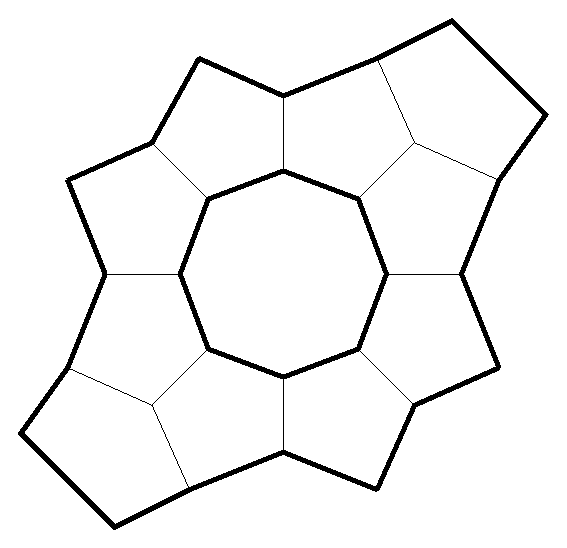
\epsfig{file=ElemPresPic/TwoHoleExample2.eps, width=5.0cm}\par
A $(\{5\}, 3)$-polycycle
\end{minipage}
\end{center}
}



\frame{
\frametitle{$(\{3\},3)$-polycycles}
Any $(\{3\},3)$-polycycle is one of the following
\begin{itemize}
\item Tetrahedron (with no hole):
\begin{center}
\epsfig{file=PictureAppli/TetrahedronSec.pdf, height=2.0cm}\par
\end{center}
\item $3$ following polycycles (with one hole):
\begin{center}
\epsfig{figure=ElemPresPic/Possible3gonal1hole.eps,width=6cm}
\end{center}
\end{itemize}
}




\frame{
\frametitle{$(\{4\},3)$-polycycles}
Any $(\{4\},3)$-polycycle is one of the following
\begin{itemize}
\item Cube (with no hole):
\begin{center}
\epsfig{file=PictureAppli/Cube.eps, height=1.5cm}\par
\end{center}
\item $3$ following polycycles (with one hole)
\begin{center}
\epsfig{figure=ElemPresPic/Possible4gonalDisc1hole.eps,width=6cm}
\end{center}
\item Following infinite family (with one hole):
\begin{center}
\epsfig{figure=ElemPresPic/Possible4gonalInfinite.eps,width=8cm}
\end{center}
\end{itemize}
}


\frame{
\frametitle{$(\{4\},3)$-polycycles}
\begin{itemize}
\item The infinite family $Prism_n$ (with two holes)
\begin{center}
\begin{minipage}[b]{2.0cm}
\centering
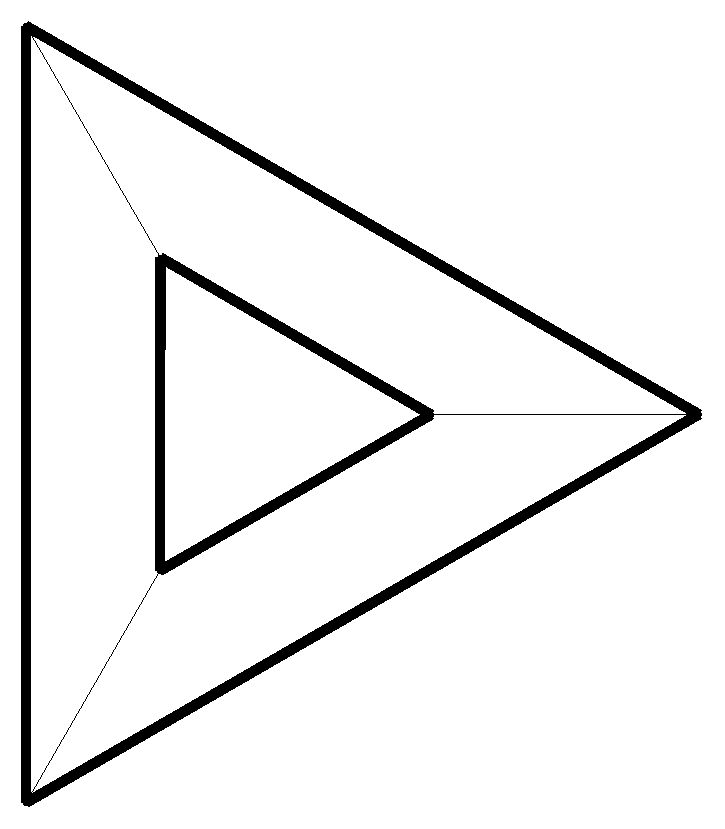
\epsfig{file=ElemPresPic/Prism3.eps, width=1.8cm}\par
\end{minipage}
\begin{minipage}[b]{2.0cm}
\centering
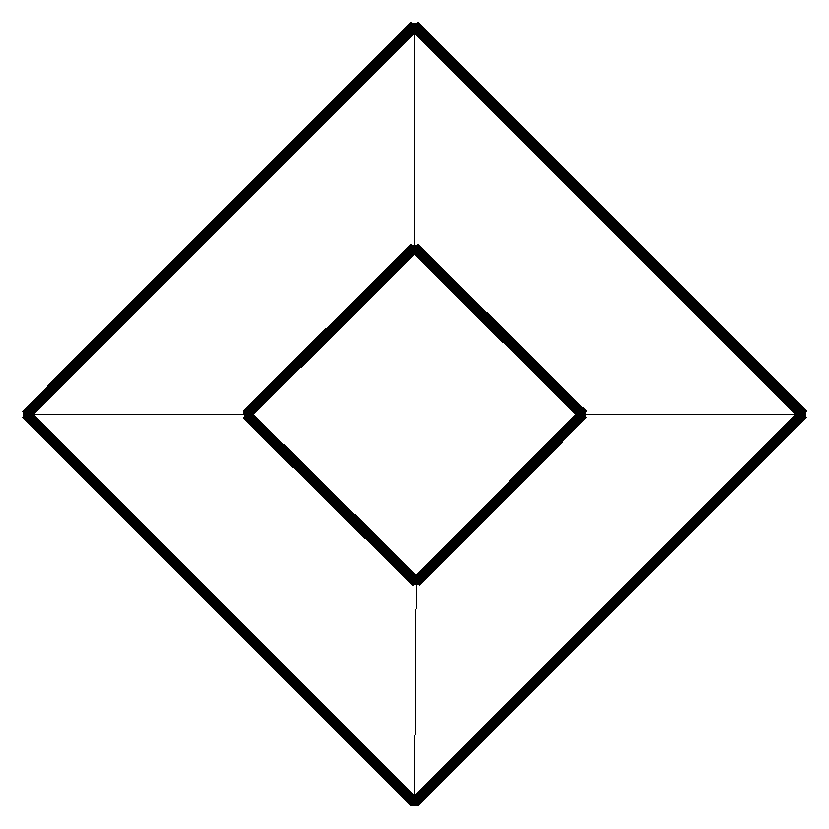
\epsfig{file=ElemPresPic/Prism4.eps, width=1.8cm}\par
\end{minipage}
\begin{minipage}[b]{2.0cm}
\centering
\epsfig{file=ElemPresPic/Prism5.eps, width=1.8cm}\par
\end{minipage}
\begin{minipage}[b]{2.0cm}
\centering
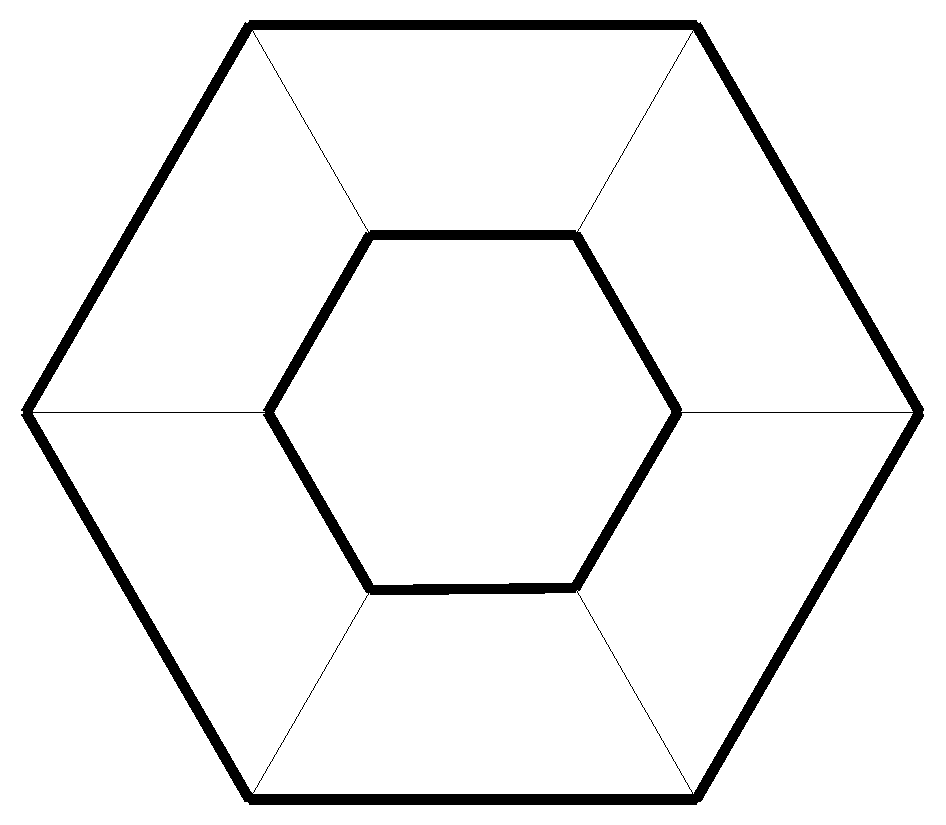
\epsfig{file=ElemPresPic/Prism6.eps, width=1.8cm}\par
\end{minipage}
\end{center}
\item Following two infinite $(\{4\},3)$-polycycles:
\begin{center}
\begin{minipage}{5.2cm}
\centering
\epsfig{height=7.5mm, file=ElemPresPic/SingleInfCube.eps}\par
singly infinite polycycle
\end{minipage}
\begin{minipage}{5.4cm}
\centering
\epsfig{height=7.5mm, file=ElemPresPic/NonExtInfCube.eps}\par
doubly infinite polycycle
\end{minipage}
\end{center}
\end{itemize}
}





\frame{
\frametitle{$(\{3\},4)$-polycycles}
\begin{itemize}
\item Octahedron (with no hole): 
\begin{center}
\epsfig{file=PictureAppli/OctahedronSec.pdf, height=1.2cm}\par
\end{center}
\item Following polycycles (with one hole)
\begin{center}
\begin{minipage}[b]{3.0cm}
\centering
\epsfig{file=ElemPresPic/34poly_1vert.eps, height=1.5cm}\par
\end{minipage}
\begin{minipage}[b]{3.0cm}
\centering
\epsfig{file=ElemPresPic/34poly_R.eps, height=1.5cm}\par
\end{minipage}
\begin{minipage}[b]{3.0cm}
\centering
\epsfig{file=ElemPresPic/34poly_RT.eps, height=1.5cm}\par
\end{minipage}
\begin{minipage}[b]{3.0cm}
\centering
\epsfig{file=ElemPresPic/4trig.eps, height=2.0cm}\par
\end{minipage}
\begin{minipage}[b]{3.0cm}
\centering
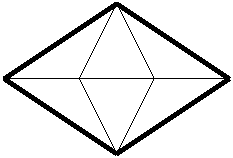
\epsfig{file=ElemPresPic/34poly_2intVert.eps, height=2.0cm}\par
\end{minipage}
\begin{minipage}[b]{3.0cm}
\centering
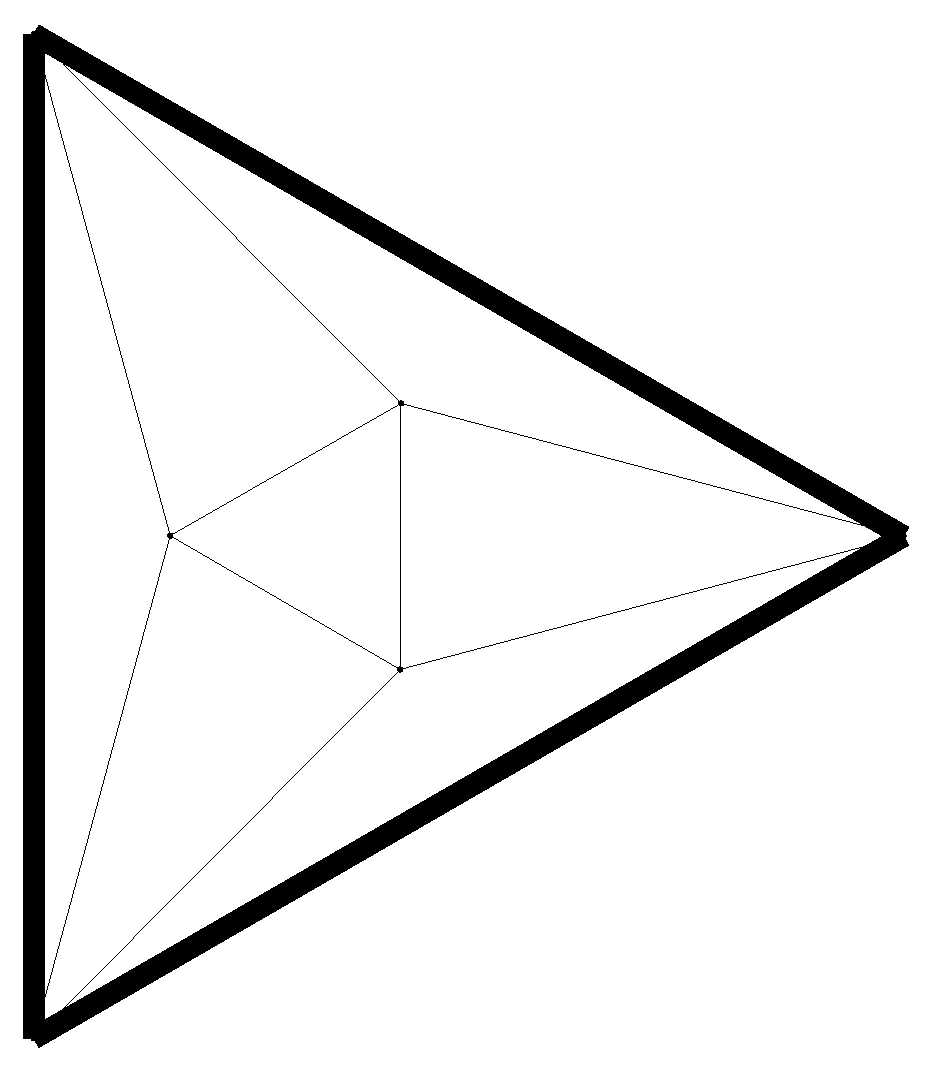
\epsfig{file=ElemPresPic/Octahedron1hole.eps, height=2.0cm}\par
\end{minipage}

\end{center}
\end{itemize}
}


\frame{
\frametitle{$(\{3\},4)$-polycycles}
\begin{itemize}
\item Following infinite family (with one hole):
\begin{center}
\epsfig{file=ElemPresPic/InfiniteFamilyTrig.eps, height=1.4cm}
\end{center}
\item The infinite family $APrism_n$ (with two holes)
\begin{center}
\begin{minipage}[b]{2.0cm}
\centering
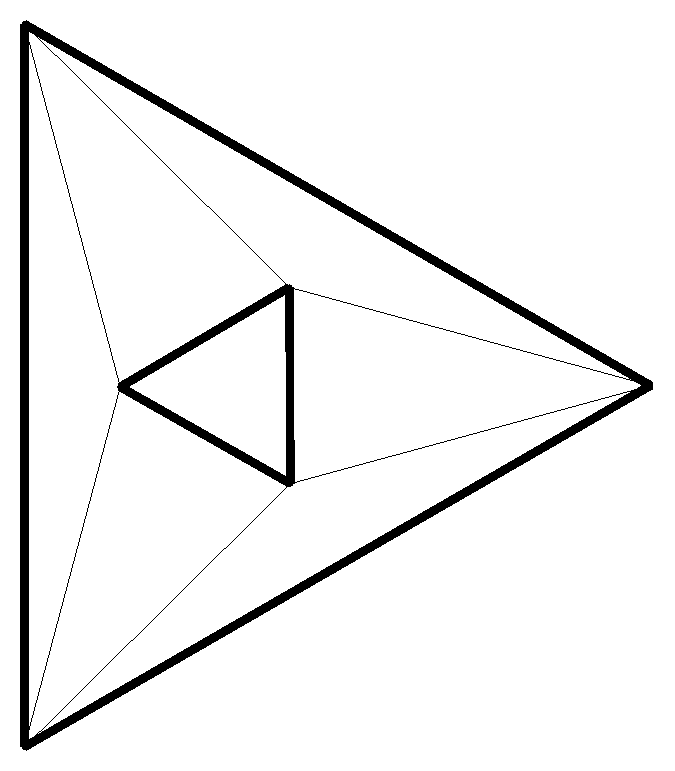
\epsfig{file=ElemPresPic/APrism3sec.eps, width=1.8cm}\par
\end{minipage}
\begin{minipage}[b]{2.0cm}
\centering
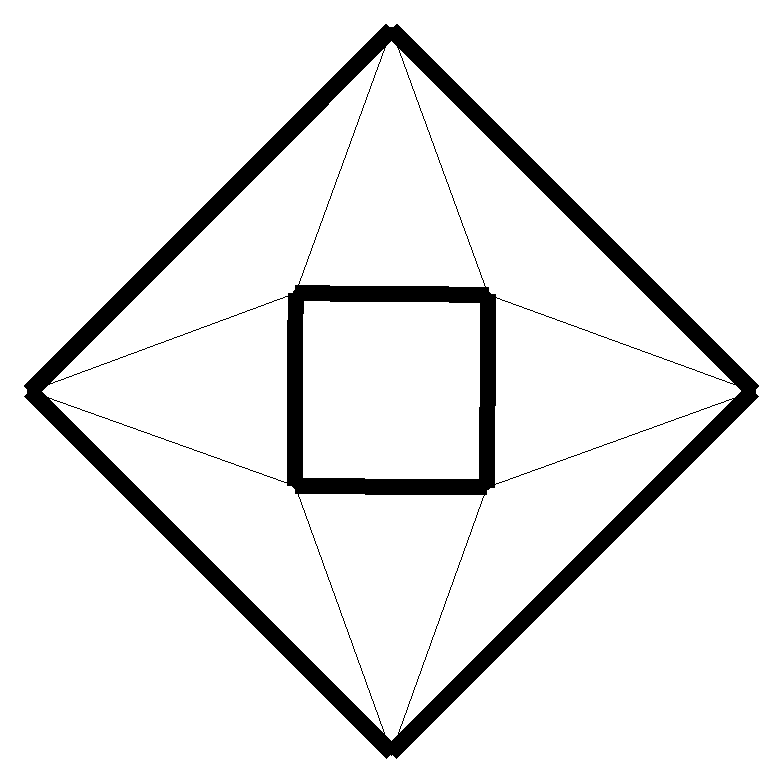
\epsfig{file=ElemPresPic/APrism4sec.eps, width=1.8cm}\par
\end{minipage}
\begin{minipage}[b]{2.0cm}
\centering
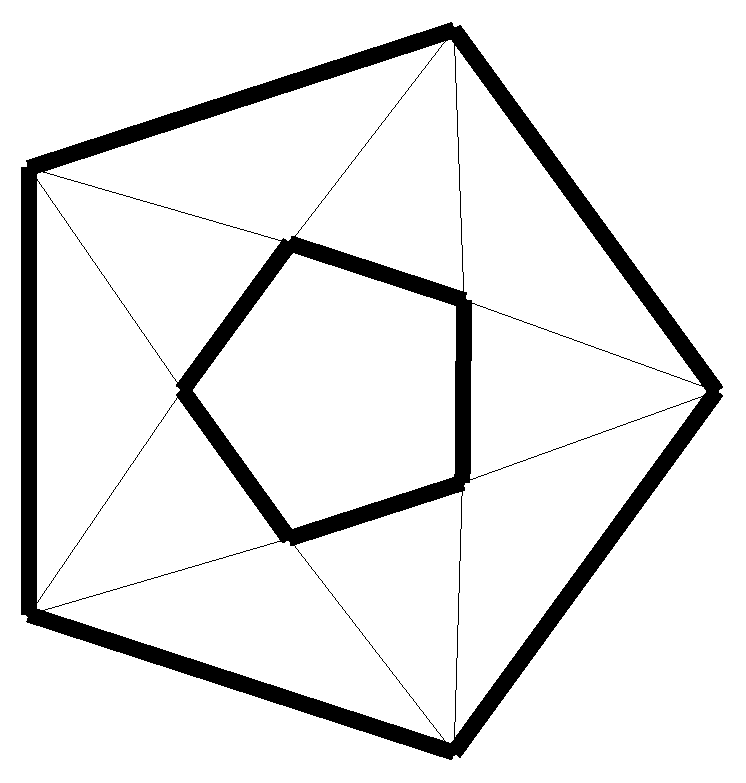
\epsfig{file=ElemPresPic/APrism5sec.eps, width=1.8cm}\par
\end{minipage}
\begin{minipage}[b]{2.0cm}
\centering
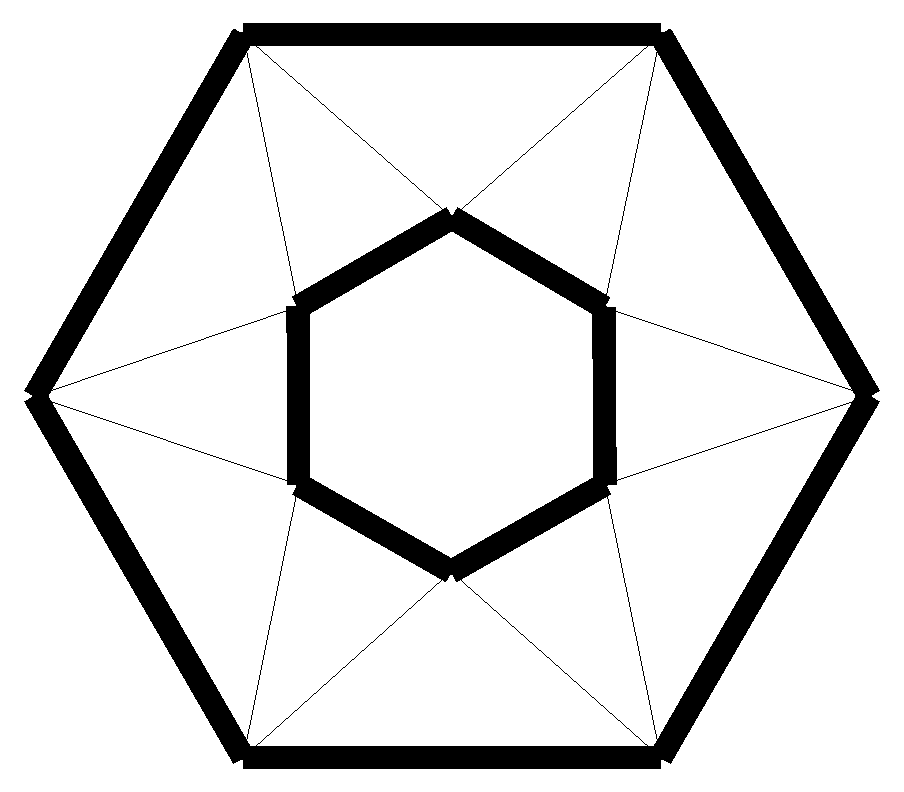
\epsfig{file=ElemPresPic/APrism6sec.eps, width=1.8cm}\par
\end{minipage}
\end{center}
\item Following two infinite $(\{3\},4)$-polycycles:
\begin{center}
\begin{minipage}{5.2cm}
\centering
\epsfig{height=7.5mm, file=ElemPresPic/SingleInfTrig.eps}\par
singly infinite polycycle
\end{minipage}
\begin{minipage}{5.4cm}
\centering
\epsfig{height=7.5mm, file=ElemPresPic/NonExtInfTrig.eps}\par
doubly infinite polycycle
\end{minipage}
\end{center}
\end{itemize}
}



\frame{
\frametitle{Curvature conditions}
\begin{itemize}
\item A $(R,q)$-polycycle is called \textcolor{red}{elliptic}, \textcolor{red}{parabolic} or \textcolor{red}{hyperbolic} if $\frac{1}{q} + \frac{1}{max_{i \in R}i} - \frac{1}{2}$ is positive, zero or negative, respectively.
\item Elliptic cases:
\begin{itemize}
\item $q=3$ and $R$ with $\max_{i\in R}i\leq 5$
\item $q=4$ and $R$ with $\max_{i\in R}i\leq 3$
\item $q=5$ and $R$ with $\max_{i\in R}i\leq 3$
\end{itemize}
\item Parabolic cases:
\begin{itemize}
\item $q=3$ and $R$ with $\max_{i\in R}i = 6$
\item $q=4$ and $R$ with $\max_{i\in R}i = 4$
\item $q=6$ and $R$ with $\max_{i\in R}i = 3$
\end{itemize}
\item All other cases are hyperbolic.
\end{itemize}
}


\frame{
\frametitle{Limit case $F_2=\emptyset$, $R=\{r\}$}
\begin{itemize}
\item Elliptic $(\{r\}, q)$-polycycles: \textcolor{red}{$5$ Platonic solids}
\begin{center}
\begin{minipage}[b]{1.9cm}
\centering
\epsfig{file=PictureAppli/TetrahedronSec.pdf, width=2.0cm}\par
Tetra-\par
hedron
\end{minipage}
\begin{minipage}[b]{1.9cm}
\centering
\epsfig{file=PictureAppli/Cube.eps, width=2.0cm}\par
Cube\par
\textcolor{white}{Bonjour}
\end{minipage}
\begin{minipage}[b]{1.9cm}
\centering
\epsfig{file=PictureAppli/OctahedronSec.pdf, width=2.0cm}\par
Octa-\par
hedron
\end{minipage}
\begin{minipage}[b]{1.9cm}
\centering
\epsfig{file=PictureAppli/Icosahedron.pdf, width=2.0cm}\par
Icosa-\par
hedron
\end{minipage}
\begin{minipage}[b]{1.9cm}
\centering
\epsfig{file=PictureAppli/Dodecahedron.eps, width=2.0cm}\par
Dodeca-\par
hedron
\end{minipage}
\end{center}
\item Parabolic $(\{r\}, q)$-polycycles: \textcolor{red}{$3$ regular plane tilings}
\begin{center}
\begin{minipage}[b]{3.0cm}
\centering

\epsfig{file=FigureWythoff/Reg1.eps, width=2.8cm}\par
\end{minipage}
\begin{minipage}[b]{3.0cm}
\centering
\epsfig{file=FigureWythoff/Reg2.eps, width=2.8cm}\par
\end{minipage}
\begin{minipage}[b]{3.0cm}
\centering
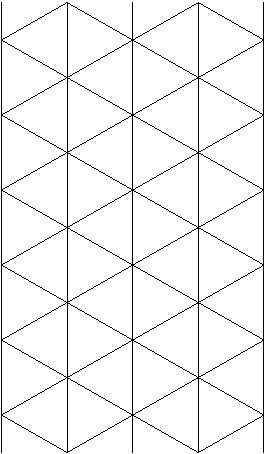
\epsfig{file=FigureWythoff/Reg3.eps, width=2.8cm}\par
\end{minipage}
\end{center}
\item Hyperbolic $(\{r\}, q)$-polycycles: \textcolor{red}{infinity}
\end{itemize}
}



\frame{
\frametitle{Generalization and $(r,q)$-polycycles}
\begin{itemize}
\item A generalization of $(R,q)$-polycycle is $(R,Q)$-polycycles: the valency of interior vertices belong to a set $Q$. All the theory extends to this case.
\item A \textcolor{red}{$(r,q)$-polycycle} is a $(\{r\}, q)$-polycycle with only one hole (the exterior one). Their theory has additional features:
\begin{itemize}
\item There exist a canonical model of them in the form of $(r^q)$ regular partition.
\item For any $(r,q)$-polycycle $P$, simple connectedness of $P$ ensures the existence of a canonical map from $P$ to $(r^q)$.
\end{itemize}
\end{itemize}
}


\frame{
\frametitle{Main examples of $(r,q)$-polycycles}
\begin{tabular}{c|c|c|c}
         &Elliptic      &Parabolic    &Hyperbolic\\
\hline
$(r,q)$  & $(3,3), (3,4), (4,3)$ & $(4,4)$ &all\\
         &   $(5,3), (3,5)$      & $(3,6), (6,3)$ &others\\
\hline
Exp.     & $\alpha_3$, $\beta_3$, $\gamma_3$, $Do$, $Ico$ &$(4^4), (6^3), (3^6)$  &$(r^q)$\\
reg.part & of sphere $S^2$     &of Euclidean    &of hyperbolic\\
         &                     &plane $\RR^2$   & plane $\HH^2$\\
\hline
\end{tabular}
\textcolor{white}{Bonjour}
\begin{center}
\epsfig{file=ElemPresPic/BasicTileObject.eps, height=1cm}
\end{center}

Polyominoes: Conway, Penrose, Colomb (games, tilers of $\RR^2$, etc.), enumeration (in Physics, Statistical Mechanics).

Polyhexes: application in Organic Chemistry.
}






\frame{
\begin{center}
{\Huge 
\begin{tabular*}{8cm}{c}
\\[-0.5cm]
\textcolor{blue}{II. }\textcolor{red}{Decomposition}\\
\textcolor{red}{into elementary}\\
\textcolor{red}{polycycles}
\end{tabular*}
}
\end{center}
}


\frame{
\frametitle{Elementary polycycles}
\begin{itemize}
\item A \textcolor{red}{bridge} of a $(R,q)$-polycycle is an edge,
which is not on a boundary and goes from a hole to a hole (possibly,
the same).
\item An \textcolor{red}{elementary $(R,q)$-polycycle} is one without bridges.
\item Examples:
\begin{center}
\begin{minipage}[b]{4.8cm}
\centering
\epsfig{file=ElemPresPic/NonElementary.eps, width=4.0cm}\par
A non-elementary $(\{4,5\},3)$-polycycle
\end{minipage}
\begin{minipage}[b]{4.8cm}
\centering
\epsfig{file=Polycycle/Elementary53_E2.eps, width=4.0cm}\par
An elementary $(\{5\},3)$-polycycle
\end{minipage}
\end{center}

\end{itemize}
}


\frame{
\frametitle{Open edges}
\begin{itemize}
\item An \textcolor{red}{open edge} of an $(R,q)$-polycycle is an edge on a boundary such that each of its end-vertices have degree less than $q$.
\item Examples
\begin{center}
\begin{minipage}[b]{4.8cm}
\centering
\epsfig{file=ElemPresPic/OpenEdge_1.eps, width=4.0cm}\par
\end{minipage}
\begin{minipage}[b]{4.8cm}
\centering
\epsfig{file=ElemPresPic/OpenEdge_2.eps, width=4.0cm}\par
\end{minipage}
\end{center}
\end{itemize}
}



\frame{
\frametitle{Decomposition theorem}
\begin{itemize}
\item \textcolor{red}{Theorem}: Any $(R,q)$-polycycle is uniquely decomposed into elementary $(R,q)$-polycycles along its bridges.
\item In other words, any $(R,q)$-polycycle is obtained by gluing some elementary $(R,q)$-polycycles along open edges.
\end{itemize}
\begin{center}
\begin{minipage}[b]{4.8cm}
\centering
\epsfig{file=FaceRegularPresPic/PolycycleFig3.eps, width=4.7cm}\par
\end{minipage}
\begin{minipage}[b]{4.8cm}
\centering
\epsfig{file=FaceRegularPresPic/PolycycleFig4.eps, width=4.7cm}\par
\end{minipage}
\end{center}

%\begin{center}
%\epsfig{file=FaceRegularPresPic/PolycycleFig3.eps, width=6cm}\par
%\end{center}
%\begin{center}
%\epsfig{file=FaceRegularPresPic/PolycycleFig4.eps, width=9cm}\par
%\end{center}
}


\frame{
\frametitle{Summary}
\begin{itemize}
\item Elementary $(R,q)$-polycycles provide a decomposition of $(R,q)$-polycycles.
\item In order for this to be useful, we have to classify the elementary $(R,q)$-polycycles.
\item For non-elliptic cases, there is no hope of classification (there is a continuum of elementary ones):
\begin{center}
\epsfig{file=ElemPresPic/NonParabolicExample.eps, width=6cm}\par
\end{center}

\end{itemize}
}



\frame{
\begin{center}
{\Huge 
\begin{tabular*}{9.5cm}{c}
\\[-0.5cm]
\textcolor{blue}{III. }\textcolor{red}{Classification}\\
\textcolor{red}{of elementary}\\
\textcolor{red}{$(\{2,3,4,5\},3)$-polycycles}
\end{tabular*}
}
\end{center}
}





\frame{
\frametitle{With at least one $2$-gon}
All elementary $(\{2,3,4,5\}, 3)$-polycycles, containing a \textcolor{red}{$2$-gon}, are those
eight ones:
\begin{center}
\begin{minipage}{2.5cm}
\centering
\epsfig{height=20mm, file=ElementaryDrawing/2gon.eps}\par
\textcolor{white}{bonjour}
\end{minipage}
\begin{minipage}{2.5cm}
\centering
\epsfig{height=20mm, file=ElementaryDrawing/El244.eps}\par
\textcolor{white}{bonjour}
\end{minipage}
\begin{minipage}{2.5cm}
\centering
\epsfig{height=20mm, file=ElementaryDrawing/El255.eps}\par
\textcolor{white}{bonjour}
\end{minipage}
\begin{minipage}{2.5cm}
\centering

\epsfig{height=20mm, file=ElementaryDrawing/El245.eps}\par
\textcolor{white}{bonjour}
\end{minipage}
\begin{minipage}{2.5cm}
\centering
\epsfig{height=20mm, file=ElementaryDrawing/El255_3.eps}\par
\textcolor{white}{bonjour}
\end{minipage}
\begin{minipage}{2.5cm}
\centering
\epsfig{height=20mm, file=ElementaryDrawing/El255_4.eps}\par
\textcolor{white}{bonjour}
\end{minipage}
\begin{minipage}{2.5cm}
\centering
\epsfig{height=20mm, file=ElementaryDrawing/El255_5.eps}\par
\textcolor{white}{bonjour}
\end{minipage}
\begin{minipage}{2.5cm}
\centering
\epsfig{height=20mm, file=ElementaryDrawing/El255_55.eps}\par
\textcolor{white}{bonjour}
\end{minipage}
\end{center}
}



\frame{
\frametitle{Totally elementary polycycle}
\begin{itemize}
\item Call an elementary $(R,3)$-polycycle \textcolor{red}{totally elementary} if, after removing any face adjacent to a hole, one obtains a non-elementary $(R,3)$-polycycle.
\item Examples:
\begin{center}
\begin{minipage}[b]{4.8cm}
\centering
\epsfig{file=ElemPresPic/TotalElementary.eps, height=4.4cm}\par
A totally elementary polycycle
\end{minipage}
\begin{minipage}[b]{4.8cm}
\centering
\epsfig{file=ElemPresPic/NonTotalElem.eps, height=4.4cm}\par
A non-totally elementary polycycle
\end{minipage}
\end{center}
\end{itemize}
}



\frame{
\frametitle{Classification result I}
Any totally elementary $(\{3,4,5\}, 3)$-polycycle is one of:
\begin{itemize}
\item[(i)] three isolated $i$-gons, $i\in \{3,4,5\}$:
\begin{center}
\begin{minipage}{3cm}
\centering
\resizebox{2.0cm}{!}{\includegraphics{ElementaryDrawing/3gon.eps}}\par
\end{minipage}
\begin{minipage}{3cm}
\centering
\resizebox{2.0cm}{!}{\includegraphics{ElementaryDrawing/4gon.eps}}\par
\end{minipage}
\begin{minipage}{3cm}
\centering
\resizebox{2.0cm}{!}{\includegraphics{ElementaryDrawing/5gon.eps}}\par
\end{minipage}
\end{center}
\item[(ii)] all ten triples of $i$-gons, $i\in \{3,4,5\}$:
\begin{center}
\begin{minipage}{2cm}
\centering
\resizebox{1.6cm}{!}{\includegraphics{ElementaryDrawing/El333.eps}}\par
\end{minipage}
\begin{minipage}{2cm}
\centering
\resizebox{1.6cm}{!}{\includegraphics{ElementaryDrawing/El334.eps}}\par
\end{minipage}
\begin{minipage}{2cm}
\centering
\resizebox{1.6cm}{!}{\includegraphics{ElementaryDrawing/El335.eps}}\par
\end{minipage}
\begin{minipage}{2cm}
\centering
\resizebox{1.6cm}{!}{\includegraphics{ElementaryDrawing/El345.eps}}\par
\end{minipage}
\begin{minipage}{2cm}
\centering
\resizebox{1.6cm}{!}{\includegraphics{ElementaryDrawing/El344.eps}}\par
\end{minipage}
\begin{minipage}{2cm}
\centering
\resizebox{1.6cm}{!}{\includegraphics{ElementaryDrawing/El355.eps}}\par
\end{minipage}
\begin{minipage}{2cm}
\centering
\resizebox{1.6cm}{!}{\includegraphics{ElementaryDrawing/El455.eps}}\par
\end{minipage}
\begin{minipage}{2cm}
\centering
\resizebox{1.6cm}{!}{\includegraphics{ElementaryDrawing/El445.eps}}\par
\end{minipage}
\begin{minipage}{2cm}
\centering
\resizebox{1.6cm}{!}{\includegraphics{ElementaryDrawing/El444.eps}}\par
\end{minipage}
\begin{minipage}{2cm}
\centering
\resizebox{1.6cm}{!}{\includegraphics{ElementaryDrawing/El555.eps}}\par
\end{minipage}

\end{center}
\end{itemize}
}

\frame{
\frametitle{Classification result II}
\begin{itemize}
\item[(iii)] the following doubly infinite $(\{5\},3)$-polycycle, denoted by $Barrel_{\infty}$:
\begin{center}
\epsfig{height=10mm, file=ElementaryDrawing/TotalElemE_Z.eps}\par
\end{center}
\item[(iv)] the infinite series of $Barrel_m$, $m\geq 2$:
\begin{center}
\begin{minipage}{2.5cm}
\centering
\epsfig{height=20mm, file=ElementaryDrawing/Barrel2sec.eps}\par
\end{minipage}
\begin{minipage}{2.5cm}
\centering
\epsfig{height=20mm, file=ElementaryDrawing/Barrel3thi.eps}\par
\end{minipage}
\begin{minipage}{2.5cm}
\centering
\epsfig{height=20mm, file=ElementaryDrawing/Barrel4thi.eps}\par
\end{minipage}
\begin{minipage}{2.5cm}
\centering
\epsfig{height=20mm, file=ElementaryDrawing/Barrel5thi.eps}\par
\end{minipage}
\end{center}

\end{itemize}
}



\frame{
\frametitle{Classification methodology}
\begin{itemize}
\item If an elementary polycycle is not totally elementary, then it is obtained from another elementary one with one face less.
\item So, from the list of elementary $(\{3,4,5\},3)$-polycycles with $n$ faces, one gets the list of elementary $(\{3,4,5\}, 3)$-polycycles with $n+1$ faces.
\begin{center}
\epsfig{height=35mm, file=ElemPresPic/ExampleGeneration_1.eps}\par
\end{center}

\end{itemize}
}



\frame{
\frametitle{Full classification}
\textcolor{red}{Theorem}: Any elementary $(\{2,3,4,5\},3)$-polycycle is one of:
\begin{itemize}
%\item eight such polycycles containing $2$-gons
%\item totally elementary polycycles
\item[(i)] $204$ sporadic polycycles with $4$ to $11$ proper faces
\item[(ii)] an element of the infinite series of $Barrel_m$, $2\leq m\leq\infty$.
\item[(iii)] six $(\{3,4,5\},3)$-polycycles, infinite in one direction:
\begin{center}
\begin{minipage}{4.8cm}
\centering
\epsfig{height=8mm, file=ElementaryDrawing/Infinite_1.eps}\par
$\alpha$
\end{minipage}
\begin{minipage}{4.8cm}
\centering
\epsfig{height=8mm, file=ElementaryDrawing/Infinite_4.eps}\par
$\delta$
\end{minipage}
\begin{minipage}{4.8cm}
\centering
\epsfig{height=8mm, file=ElementaryDrawing/Infinite_2.eps}\par
$\beta$
\end{minipage}
\begin{minipage}{4.8cm}
\centering
\epsfig{height=8mm, file=ElementaryDrawing/Infinite_5.eps}\par
$\varepsilon$
\end{minipage}
\begin{minipage}{4.8cm}
\centering
\epsfig{height=8mm, file=ElementaryDrawing/Infinite_3.eps}\par
$\gamma$
\end{minipage}
\begin{minipage}{4.8cm}
\centering
\epsfig{height=8mm, file=ElementaryDrawing/Infinite_6.eps}\par
$\mu$
\end{minipage}
\end{center}
\end{itemize}
}

\frame{
\begin{itemize}
\item[(iv)] $21={{6+1}\choose 2}$ infinite series obtained by taking two 
endings of the above infinite polycycles and concatenating them.\\[3mm]
See below three examples in the infinite series $\beta\varepsilon$
\begin{itemize}
\item 
\begin{center}
\begin{minipage}{30mm}
\centering
\epsfig{height=11mm, file=ElementaryDrawing/BetaEpsilonSerie_1.eps}\par
\end{minipage}
\end{center}

\item 
\begin{center}
\begin{minipage}{35mm}
\centering
\epsfig{height=11mm, file=ElementaryDrawing/BetaEpsilonSerie_2.eps}\par
\end{minipage}
\end{center}


\item 
\begin{center}
\begin{minipage}{40mm}
\centering
\epsfig{height=11mm, file=ElementaryDrawing/BetaEpsilonSerie_3.eps}\par
\end{minipage}
\end{center}

\end{itemize}

\end{itemize}
}


\frame{
\frametitle{Subcase of $(\{5\},3)$-polycycles}
%\textcolor{red}{Thm.}
\begin{itemize}
\item[(i)] Sporadic elementary $(\{5\},3)$-polycycles:
\end{itemize}
\begin{center}
\begin{minipage}[b]{2.6cm}
\centering
\resizebox{2.0cm}{!}{\includegraphics{PictureAppli/Dodecahedron.eps}}\par
$A_1$
\end{minipage}
\begin{minipage}[b]{2.6cm}
\centering
\resizebox{2.5cm}{!}{\rotatebox{90}{\includegraphics{Polycycle/PolycycleA2.eps}}}\par
$A_2$
\end{minipage}
\begin{minipage}[b]{2.6cm}
\centering
\resizebox{1.8cm}{!}{\includegraphics{Polycycle/Dodecahedron3vertDegTwoSec.pdf}}\par
$A_3$
\end{minipage}
\begin{minipage}[b]{2.6cm}
\centering
\resizebox{2.5cm}{!}{\includegraphics{Polycycle/PolycycleA4.eps}}\par
$A_4$
\end{minipage}
\begin{minipage}[b]{2.6cm}
\centering
\resizebox{2.0cm}{!}{\rotatebox{90}{\includegraphics{Polycycle/PolycycleB3sec.eps}}}\par
$B_3$
\end{minipage}
\begin{minipage}[b]{2.6cm}
\centering
\resizebox{1.8cm}{!}{\includegraphics{Polycycle/PolycycleA5.eps}}\par
$A_5$
\end{minipage}
\begin{minipage}[b]{2.6cm}
\centering
\resizebox{2.5cm}{!}{\includegraphics{Polycycle/Fundamental22polycycle3.eps}}\par
$C_1$
\end{minipage}
\begin{minipage}[b]{2.6cm}
\centering
\resizebox{2.5cm}{!}{\includegraphics{Polycycle/PolycycleB2.eps}}\par
$B_2$
\end{minipage}
\begin{minipage}[b]{2.6cm}
\centering
\resizebox{2.5cm}{!}{\includegraphics{Polycycle/Elementary53_C2.eps}}\par
$C_2$
\end{minipage}
\begin{minipage}[b]{2.6cm}
\centering
\resizebox{2.5cm}{!}{\includegraphics{Polycycle/Fundamental22polycycle2.eps}}\par
$C_3$
\end{minipage}
\begin{minipage}[b]{2.6cm}
\centering
\resizebox{2.5cm}{!}{\rotatebox{180}{\includegraphics{Polycycle/PolycycleD.eps}}}\par
$D$
\end{minipage}




\end{center}
}


\frame{
\begin{itemize}
\item[(ii)] The \textcolor{red}{infinite series} of elementary
$(\{5\},3)$-polycycles $\alpha\alpha$:\\[1cm]
\begin{center}
\begin{minipage}{2.6cm}
\centering
\epsfig{height=14mm, file=Polycycle/Elementary53_E1.eps}\par
$E_1$
\end{minipage}
\begin{minipage}{2.6cm}
\centering
\epsfig{height=14mm, file=Polycycle/Elementary53_E2.eps}\par
$E_2$
\end{minipage}
\begin{minipage}{2.6cm}
\centering
\epsfig{height=14mm, file=Polycycle/Elementary53_E3.eps}\par
$E_3$
\end{minipage}
%\begin{minipage}{2.6cm}
%\centering
%\epsfig{height=14mm, file=Polycycle/Elementary53_E4.eps}\par
%$E_4$
%\end{minipage}
%\begin{minipage}{4.7cm}
%\centering
%\epsfig{height=14mm, file=Polycycle/Elementary53_E5.eps}\par
%\end{minipage}
\end{center}
\item[(iii)] The \textcolor{red}{infinite series} of elementary
$(\{5\},3)$-polycycles $Barrel_q$, $q \ge 3$:
\begin{center}
\begin{minipage}{2.6cm}
\centering
\epsfig{height=22mm, file=FaceRegularPresPic/Barrel3sec.eps}\par
\end{minipage}
\begin{minipage}{2.6cm}
\centering
\epsfig{height=22mm, file=FaceRegularPresPic/Barrel4sec.eps}\par
\end{minipage}
\begin{minipage}{2.6cm}
\centering
\epsfig{height=22mm, file=ElemPresPic/Barrel5.eps}\par
\end{minipage}
%\begin{minipage}{2.6cm}
%\centering
%\epsfig{height=22mm, file=FaceRegularPresPic/G1sec.eps}\par
%\end{minipage}
%\begin{minipage}{5.0cm}
%\centering
%\epsfig{height=34mm, file=FaceRegularPresPic/G2sec.eps}\par
%\end{minipage}
\end{center}
\item[(iv)] The only elementary \textcolor{red}{infinite} $(\{5\},3)$-polycycle
are $Barrel_{\infty}$ and $\alpha$
\end{itemize}
}


\frame{
\begin{center}
{\Huge 
\begin{tabular*}{8cm}{c}
\\[-0.5cm]
\textcolor{blue}{IV. }\textcolor{red}{Classification}\\
\textcolor{red}{of elementary}\\
\textcolor{red}{$(\{2,3\},4)$-polycycles}
\end{tabular*}
}
\end{center}
}


\frame{
\frametitle{The classification}
Any elementary $(\{2,3\}, 4)$-polycycle is one of the following eight:

\begin{center}
\begin{minipage}{2.5cm}
\centering
\resizebox{2.0cm}{!}{\includegraphics{ElementaryDrawing/3gon.eps}}\par
\end{minipage}
\begin{minipage}{2.5cm}
\centering
\epsfig{height=20mm, file=ElementaryDrawing/El4_4.eps}\par
\end{minipage}
\begin{minipage}{3.0cm}
\centering
\epsfig{height=20mm, file=ElementaryDrawing/El4_6.eps}\par
\end{minipage}
\begin{minipage}{2.5cm}
\centering
\resizebox{20mm}{!}{\rotatebox{0}{\includegraphics{ElementaryDrawing/Octahedron3vert.eps}}}\par
\end{minipage}
\begin{minipage}{2.5cm}
\centering
\epsfig{height=20mm, file=ElementaryDrawing/2gon.eps}\par
\end{minipage}
\begin{minipage}{2.5cm}
\centering
\epsfig{height=20mm, file=ElementaryDrawing/El4_2333.eps}\par
\end{minipage}
\begin{minipage}{2.5cm}
\centering
\epsfig{height=20mm, file=ElementaryDrawing/El4_23333.eps}\par
\end{minipage}
\begin{minipage}{2.5cm}
\centering
\epsfig{height=20mm, file=ElementaryDrawing/El4_2233.eps}\par
\end{minipage}
\end{center}
}




\frame{
\begin{center}
{\Huge 
\begin{tabular*}{8cm}{c}
\\[-0.5cm]
\textcolor{blue}{V. }\textcolor{red}{Classification}\\
\textcolor{red}{of elementary}\\
\textcolor{red}{$(\{2,3\},5)$-polycycles}
\end{tabular*}
}
\end{center}
}

\frame{
\frametitle{The technique}
\begin{itemize}
\item Take an elementary $(\{2,3\},5)$-polycycle. If $v$ is a vertex on the boundary, then we can consider all possible ways to make this vertex an interior vertex in an elementary $(\{2,3\}, 5)$-polycycle.
\item From the list of elementary $(\{2,3\}, 5)$-polycycles with $n$ interior vertices, one can obtain the list of elementary $(\{2,3\}, 5)$-polycycles with $n+1$ interior vertices.
\begin{center}
\epsfig{height=35mm, file=ElemPresPic/VertexExtension.eps}\par
\end{center}
\end{itemize}
}






\frame{
\frametitle{The classification}
Any elementary $(\{2,3,4,5\},3)$-polycycle is one of:
\begin{itemize}
\item[(i)] $57$ sporadic $(\{2,3\},5)$-polycycles.

\item[(ii)] three following infinite $(\{2,3\},5)$-polycycles:
\begin{center}
\begin{minipage}{1cm}
$\alpha$:
\end{minipage}
\begin{minipage}{8cm}
\centering
\resizebox{8.0cm}{!}{\rotatebox{180}{\includegraphics{ElementaryDrawing/5valInfinite2.eps}}}\par
\end{minipage}
\begin{minipage}{10cm}
\textcolor{white}{Bonjour, ici la terre}
\end{minipage}
\begin{minipage}{1cm}
$\beta$:
\end{minipage}
\begin{minipage}{8cm}
\centering
\resizebox{8.0cm}{!}{\rotatebox{180}{\includegraphics{ElementaryDrawing/5valInfinite3.eps}}}\par
\end{minipage}
\begin{minipage}{10cm}
\textcolor{white}{Bonjour, ici la terre}
\end{minipage}
\begin{minipage}{1cm}
$\gamma$:
\end{minipage}
\begin{minipage}{8cm}
\centering
\resizebox{8.0cm}{!}{\rotatebox{180}{\includegraphics{ElementaryDrawing/5valInfinite4.eps}}}\par
\end{minipage}
\end{center}
\end{itemize}
}

\frame{
\begin{itemize}
\item[(iii)] the following $5$-valent doubly infinite
$(\{2,3\},5)$-polycycle, called \textcolor{red}{snub $\infty$-antiprism}:
\begin{center}
\begin{minipage}{8cm}
\centering
\epsfig{height=10mm, file=ElementaryDrawing/5valInfinite1.eps}\par
\end{minipage}
\end{center}

\item[(iv)] the infinite series of \textcolor{red}{snub $m$-antiprisms},
$m\geq 2$ (two $m$-gonal holes):
\begin{center}
\begin{minipage}{2.5cm}
\centering
\epsfig{height=20mm, file=ElementaryDrawing/5valSer2sec.eps}\par
\end{minipage}
\begin{minipage}{2.5cm}
\centering
\epsfig{height=20mm, file=ElementaryDrawing/5valSer3sec.eps}\par
\end{minipage}
\begin{minipage}{2.5cm}
\centering
\epsfig{height=20mm, file=ElementaryDrawing/5valSer4sec.eps}\par
\end{minipage}
\begin{minipage}{2.5cm}
\centering
\epsfig{height=20mm, file=ElementaryDrawing/5valSer5sec.eps}\par
\end{minipage}
%\begin{minipage}{3cm}
%\centering
%\epsfig{height=20mm, file=ElementaryDrawing/5valSer6sec.eps}\par
%$D_{6d}$
%\end{minipage}
\end{center}

\item[(v)] six infinite series of $(\{2,3\},5)$-polycycles with one hole
(they are obtained by concatenating endings $\alpha$, $\beta$, $\gamma$)

\end{itemize}
}

%\frame{
%Infinite series $\alpha\gamma$ of elementary $(\{2,3\},5)$-polycycles:
%\begin{center}
%\begin{minipage}{3cm}
%\centering
%\epsfig{height=17mm, file=ElementaryDrawing/5_val2ver_5.eps}\par
%\end{minipage}
%\begin{minipage}{3cm}
%\centering
%\epsfig{width=28mm, file=ElementaryDrawing/5_val3ver_5.eps}\par
%\end{minipage}
%\begin{minipage}{3cm}
%\centering
%\epsfig{width=28mm, file=ElementaryDrawing/5_val4ver_7.eps}\par
%\end{minipage}
%\begin{minipage}{3cm}
%\centering
%\epsfig{width=28mm, file=ElementaryDrawing/5_val5ver_8.eps}\par
%\end{minipage}
%\begin{minipage}{3cm}
%\centering
%\epsfig{width=28mm, file=ElementaryDrawing/5_val6ver_9.eps}\par
%\end{minipage}
%\end{center}
%Infinite series $\beta\gamma$ of elementary $(\{2,3\},5)$-polycycles:
%\begin{center}
%\begin{minipage}{3cm}
%\centering
%\epsfig{height=16mm, file=ElementaryDrawing/5_val2ver_7.eps}\par
%\end{minipage}
%\begin{minipage}{3cm}
%\centering
%\epsfig{width=28mm, file=ElementaryDrawing/5_val3ver_10.eps}\par
%\end{minipage}
%\begin{minipage}{3cm}
%\centering
%\epsfig{width=28mm, file=ElementaryDrawing/5_val4ver_16.eps}\par
%\end{minipage}
%\begin{minipage}{3cm}
%\centering
%\epsfig{width=28mm, file=ElementaryDrawing/5_val5ver_14.eps}\par
%\end{minipage}
%\begin{minipage}{3cm}
%\centering
%\epsfig{width=28mm, file=ElementaryDrawing/5_val6ver_14.eps}\par
%\end{minipage}
%\end{center}
%}






\frame{
\frametitle{Subcase of $(\{3\}, 5)$-polycycles I}
\begin{itemize}
\item[(i)] Sporadic elementary $(\{3\}, 5)$-polycycles:
\end{itemize}
\begin{center}
\begin{minipage}{3cm}
\centering
\resizebox{2.0cm}{!}{\includegraphics{ElementaryDrawing/3gon.eps}}\par
\end{minipage}
\begin{minipage}{3cm}
\centering
\epsfig{width=25mm, file=ElementaryDrawing/5_val3ver_1.eps}\par
\end{minipage}
\begin{minipage}{3cm}
\centering
\epsfig{width=28mm, file=ElementaryDrawing/5_val4ver_2.eps}\par
\end{minipage}
\begin{minipage}{3cm}
\centering
\epsfig{width=28mm, file=ElementaryDrawing/5_val4ver_1.eps}\par
\end{minipage}
\begin{minipage}{3cm}
\centering
\epsfig{width=28mm, file=ElementaryDrawing/5_val5ver_1.eps}\par
\end{minipage}
\begin{minipage}{3cm}
\centering
\epsfig{width=28mm, file=ElementaryDrawing/5_val5ver_2.eps}\par
\end{minipage}
\begin{minipage}{3cm}
\centering
\epsfig{width=28mm, file=ElementaryDrawing/5_val6ver_1.eps}\par
\end{minipage}
\begin{minipage}{3cm}
\centering
\epsfig{width=28mm, file=ElementaryDrawing/5_val6ver_2.eps}\par
\end{minipage}
\begin{minipage}{3cm}
\centering
\epsfig{width=24mm, file=ElementaryDrawing/5_val6ver_4.eps}\par
\end{minipage}

\end{center}
}

\frame{
\frametitle{Subcase of $(\{3\}, 5)$-polycycles II}
\begin{center}
\begin{minipage}{2.6cm}
\centering
\epsfig{width=25mm, file=ElementaryDrawing/5_val6ver_3.eps}\par
\end{minipage}
\begin{minipage}{2.6cm}
\centering
\epsfig{width=25mm, file=ElementaryDrawing/5_val7ver_1.eps}\par
\end{minipage}
\begin{minipage}{2.6cm}
\centering
\epsfig{width=25mm, file=ElementaryDrawing/5_val8ver_1.eps}\par
\end{minipage}
\begin{minipage}{2.6cm}
\centering
\epsfig{width=25mm, file=ElementaryDrawing/5_val9ver_1.eps}\par
\end{minipage}
\end{center}
\begin{itemize}
\item[(ii)] The \textcolor{red}{infinite series} of elementary
$(\{3\},5)$-polycycles $\alpha\alpha$:
\begin{center}
\begin{minipage}{2cm}
\centering
\epsfig{height=15mm, file=ElementaryDrawing/5_val1ver_1.eps}\par
\end{minipage}
\begin{minipage}{2cm}
\centering
\epsfig{height=17mm, file=ElementaryDrawing/5_val2ver_4.eps}\par
\end{minipage}
\begin{minipage}{3cm}
\centering
\epsfig{width=28mm, file=ElementaryDrawing/5_val3ver_2.eps}\par
\end{minipage}
\begin{minipage}{3cm}
\centering
\epsfig{width=28mm, file=ElementaryDrawing/5_val4ver_3.eps}\par
\end{minipage}
\begin{minipage}{3cm}
\centering
\epsfig{width=28mm, file=ElementaryDrawing/5_val5ver_3.eps}\par
\end{minipage}
\begin{minipage}{3cm}
\centering
\epsfig{width=28mm, file=ElementaryDrawing/5_val6ver_5.eps}\par
\end{minipage}
\end{center}
\item[(iii)] The only elementary \textcolor{red}{infinite} $(\{3\},5)$-polycycles
are $\alpha$ and snub $\infty$-antiprism.
\item[(iv)] The \textcolor{red}{infinite series} of elementary
$(\{3\},5)$-polycycles snub $m$-antiprisms, $m\geq 2$:
\end{itemize}
}




\frame{
\begin{center}
{\Huge 
\begin{tabular*}{6.5cm}{c}
\\[-0.5cm]
\textcolor{blue}{VI. }\textcolor{red}{Application}\\
\textcolor{red}{to extremal}\\
\textcolor{red}{polycycles}
\end{tabular*}
}
\end{center}
}



\frame{
\frametitle{Definition}
\begin{itemize}
\item Given a finite $(r,q)$-polycycle $P$, denote by 
\begin{itemize}
\item $n_{int}(P)$ the number of interior vertices
\item and $f_1(P)$ the number of faces in $F_1$.
\end{itemize}
\item Fix $x\in \NN$. An $(r,q)$-polycycle with $f_1(P)=x$ is called \textcolor{red}{extremal} if it has maximal $n_{int}(P)$ among all $(r,q)$-polycycles with $f_1(P)=x$.
\item \textcolor{red}{Problem}: to find $N_{r,q}(x)$, the maximal number of vertices.
\item \textcolor{red}{Fact}: For fixed $r, q, f_{1}(P)=x$  extremal polycycle
has also maximal $n_{int}(P)$, $e_{int}(P)$ (interior faces) and minimal $n$, $l$, $Perim=n_{ext}$
\item For $(r,q)$=$(3,3)$, $(4,3)$, $(3,4)$, the question is trivial.\\
$8$ authors, 1997: found $N_{5,3}(x)$ for $x < 12$ (unique, partial subgraph of Dodecahedron).
\end{itemize}
}

\frame{
\frametitle{Use of elementary polycycles}
\begin{itemize}
\item If a $(r,q)$-polycycle $P$ is decomposed into elementary $(r,q)$-polycycles $(EP_i)_{i\in I}$ appearing $x_i$ times, then one has:
\begin{equation*}
\left\lbrace\begin{array}{rcl}
n_{int}(P)&=&\sum_{i\in I} x_i n_{int}(EP_i)\\
f_{1}(P)&=&\sum_{i\in I} x_i f_{1}(EP_i)
\end{array}\right.
\end{equation*}
\item If one solves the Linear Programming problem 
\begin{equation*}
\begin{array}{rl}
\mbox{maximize}&\sum_{i\in I} x_i n_{int}(EP_i)\\
\mbox{with}&x=\sum_{i\in I} x_i f_{1}(EP_i)\\
           &\mbox{and~~}x_i\in \NN
\end{array}
\end{equation*}
and if $(x_i)_{i\in I}$ realizing the maximum can be realized as $(r,q)$-polycycle, then $N_{r,q}(x)$ can be found.
\end{itemize}
}



\frame{
\frametitle{Small extremal $(5,3)$-polycycles}
\begin{center}
\begin{tabular}{|c|c|c|c|}
\hline
$x$   &  $N_{5,3}(x)$ &extremal   & components\\
\hline
1     &  0&\epsfig{height=10mm, file=Polycycle/PolycycleD.eps}&$D$\\[2mm]\hline
2     &  0&\epsfig{height=10mm, file=Sph57/Special7R5_Nr2.eps}&$D,D$\\[2mm]\hline
3     &  1&\epsfig{height=10mm, file=Polycycle/Fundamental22polycycle1.eps}&$E_1$\\[2mm]\hline
4     &  2&\epsfig{height=10mm, file=Polycycle/Elementary53_E2.eps}&$E_2$\\[2mm]\hline
5     &  3&\epsfig{height=10mm, file=Polycycle/Elementary53_E3.eps}&$E_3$\\[2mm]\hline
\end{tabular}
\end{center}
}


\frame{
\begin{center}
\begin{tabular}{|c|c|c|c|}
\hline
$x$   &  $N_{5,3}(x)$ &extremal   & components\\
\hline
6     &  5&\epsfig{height=10mm, file=Polycycle/PolycycleA5.eps}&$A_5$\\[2mm]\hline
7     &  6&\epsfig{height=10mm, file=Polycycle/PolycycleB3sec.eps}&$B_3$\\[2mm]\hline
8     &  8&\epsfig{height=10mm, file=Polycycle/PolycycleA4.eps}&$A_4$\\[2mm]\hline
9     & 10&\epsfig{height=10mm, file=Polycycle/Dodecahedron3vertDegTwo.pdf}&$A_3$\\[2mm]\hline
10    & 12&\epsfig{height=10mm, file=Polycycle/PolycycleA2.eps}&$A_2$\\[2mm]\hline
\end{tabular}
\end{center}
}

\frame{
\begin{center}
\begin{tabular}{|c|c|c|c|}
\hline
$x$   &  $N_{5,3}(x)$ &extremal   & components\\
\hline
11    & 15&\epsfig{height=10mm, file=PictureAppli/Dodecahedron.eps}&$A_1$\\[2mm]\hline
12    & 10&\epsfig{height=10mm, file=ElemPresPic/PolycycleB2_E1.eps}&$E_1, B_2$\\[2mm]
      &   &\epsfig{height=10mm, file=ElemPresPic/PolycycleC1_2D_1.eps}&$D, C_1,D$\\[2mm]
      &   &\epsfig{height=10mm, file=ElemPresPic/PolycycleC1_2D_2.eps}&$C_1,D,D$\\[2mm]
      &   &\epsfig{height=8mm, file=Polycycle/Elementary53_E10.eps}&$E_{10}$\\[2mm]
\hline
\end{tabular}
\end{center}
}



\frame{
\frametitle{Extremal $(5,3)$-polycycles}
\begin{itemize}
%\item Polycycle $A_1$, $A_2$, $A_3$ have higher $\frac{n_{int}(P)}{f_1(P)}$ than $C_1$.
%\item But one cannot glue them with other polycycles. So, they do yield extremal polycycles for $x\geq 12$.
\item \textcolor{red}{Theorem}: For any $x\geq 12$, one has
\begin{equation*}
N_{5,3}(x)=\left\lbrace\begin{array}{lcl}
x    &if & x\equiv 0, 8, 9\pmod {10},\\
x-1  &if & x\equiv 6, 7\pmod {10},\\
x-2  &if & x\equiv 1,2,3,4,5\pmod {10}.
\end{array}\right.
\end{equation*}
\item Extremal polycycle realizing the extremum:
\begin{itemize}
\item If $x\equiv 0\pmod {10}$ (unique):
\begin{center}
\begin{minipage}{2.0cm}
\centering
\epsfig{width=21.3mm, file=Polycycle/Fundamental22polycycle3.eps}\par
\end{minipage}
\begin{minipage}{2.0cm}
\centering
\epsfig{width=20mm, file=ElemPresPic/JoinSign.eps}\par
\end{minipage}
\begin{minipage}{2.0cm}
\centering
\epsfig{width=21.3mm, file=Polycycle/Fundamental22polycycle3.eps}\par
\end{minipage}
\begin{minipage}{2.0cm}
\centering
\epsfig{width=21.3mm, file=Polycycle/Fundamental22polycycle3.eps}\par
\end{minipage}
\end{center}
\item If $x\equiv 9\pmod {10}$ (unique):
\begin{center}
\begin{minipage}{2.0cm}
\centering
\epsfig{width=21.3mm, file=Polycycle/Fundamental22polycycle3.eps}\par
\end{minipage}
\begin{minipage}{2.0cm}
\centering
\epsfig{width=20mm, file=ElemPresPic/JoinSign.eps}\par
\end{minipage}
\begin{minipage}{2.0cm}
\centering
\epsfig{width=21.3mm, file=Polycycle/Fundamental22polycycle3.eps}\par
\end{minipage}
\begin{minipage}{2.0cm}
\centering
\epsfig{width=20mm, file=Polycycle/PolycycleB2.eps}\par
\end{minipage}
\end{center}
\end{itemize}

\end{itemize}
}

\frame{
\begin{itemize}
\item Extremal polycycle realizing the extremum:
\begin{itemize}
\item If $x\equiv 8\pmod {10}$ (unique):
\begin{center}
\hspace{-10mm}
\begin{minipage}{1.9cm}
\centering
\resizebox{19mm}{!}{\rotatebox{180}{\includegraphics{Polycycle/PolycycleB2.eps}}}\par
\end{minipage}
\begin{minipage}{1.9cm}
\centering
\epsfig{width=20.3mm, file=Polycycle/Fundamental22polycycle3.eps}\par
\end{minipage}
\begin{minipage}{1.9cm}
\centering
\epsfig{width=19mm, file=ElemPresPic/JoinSign.eps}\par
\end{minipage}
\begin{minipage}{1.9cm}
\centering
\epsfig{width=20.3mm, file=Polycycle/Fundamental22polycycle3.eps}\par
\end{minipage}
\begin{minipage}{1.9cm}
\centering
\epsfig{width=19mm, file=Polycycle/PolycycleB2.eps}\par
\end{minipage}
\end{center}
\item If $x\equiv 7\pmod {10}$ (non-unique):
\begin{center}
\begin{minipage}{1.9cm}
\centering
\epsfig{width=21.3mm, file=Polycycle/Fundamental22polycycle3.eps}\par
\end{minipage}
\begin{minipage}{1.9cm}
\centering
\epsfig{width=20mm, file=ElemPresPic/JoinSign.eps}\par
\end{minipage}
\begin{minipage}{1.9cm}
\centering
\epsfig{width=21.3mm, file=Polycycle/Fundamental22polycycle3.eps}\par
\end{minipage}
\begin{minipage}{0.95cm}
\centering
\resizebox{0.75cm}{!}{\rotatebox{180}{\includegraphics{Polycycle/PolycycleB3sec.eps}}}\par
\end{minipage}
\end{center}
\item If $x\equiv 6\pmod {10}$ (non-unique):
\begin{center}
\hspace{-10mm}
\begin{minipage}{2.0cm}
\centering
\resizebox{2.0cm}{!}{\rotatebox{180}{\includegraphics{Polycycle/PolycycleB2.eps}}}\par
\end{minipage}
\begin{minipage}{2.0cm}
\centering
\epsfig{width=21.3mm, file=Polycycle/Fundamental22polycycle3.eps}\par
\end{minipage}
\begin{minipage}{2.0cm}
\centering
\epsfig{width=20mm, file=ElemPresPic/JoinSign.eps}\par
\end{minipage}
\begin{minipage}{2.0cm}
\centering
\epsfig{width=21.3mm, file=Polycycle/Fundamental22polycycle3.eps}\par
\end{minipage}
\begin{minipage}{0.75cm}
\centering
\resizebox{0.75cm}{!}{\rotatebox{180}{\includegraphics{Polycycle/PolycycleB3sec.eps}}}\par
\end{minipage}
\end{center}
\item Otherwise (non-unique): $E_n$

\end{itemize}




\end{itemize}
}


\frame{
\frametitle{Extremal $(3,5)$-polycycles}
\textcolor{red}{Theorem}
\begin{itemize}
\item $N_{3,5}(x)= \lfloor \frac{x}{3} \rfloor +1$ for $x\equiv 14,16,17 \pmod {18}$,
\item $N_{3,5}(x)= \lfloor \frac{x}{3} \rfloor -1$ for $x\equiv 3,4,6,7,9,11 \pmod {18}$, and
\item $N_{3,5}(x)= \lfloor \frac{x}{3} \rfloor$, otherwise,
\item but with $5$ exceptions: above value plus $1$ for $x=11,15,17$
and $N_{3,5}(x)=x-10$ for $16 \le x \le 19$.
\end{itemize}
}



\frame{
\frametitle{Non-elliptic case}
\begin{itemize}
\item For parabolic $(r,q)$-polycycles (i.e. $(r,q)$=$(4,4)$, $(6,3)$ or $(3,6)$) the method of elementary polycycles fails (since there is no classification) but ``extremal animals'' of Harary-Harborth 1976 (proper ones, growing as a spiral) are extremal:
\begin{center}
\epsfig{height=35mm, file=ElemPresPic/HararyHazborth.eps}\par
\end{center}
\item Hyperbolic cases are very difficult.
\end{itemize}
}


\frame{
\begin{center}
{\Huge 
\begin{tabular*}{8cm}{c}
\\[-0.5cm]
\textcolor{blue}{VII. }\textcolor{red}{Application}\\
\textcolor{red}{to non-extendible}\\
\textcolor{red}{polycycles}
\end{tabular*}
}
\end{center}
}


\frame{
\frametitle{Definition}
\begin{itemize}
\item A $(r,q)$-polycycle is called \textcolor{red}{non-extendible} if it is no proper subgraph of another $(r,q)$-polycycle. Examples:
\end{itemize}
\begin{center}
\epsfig{height=18mm, file=ElemPresPic/ExampleExtendible.eps}\par
\begin{flushleft}
Extendible $(3,4)$-polycycle
\end{flushleft}
\epsfig{height=18mm, file=ElemPresPic/ExampleNonExt.eps}\par
Non-extendible $(3,3)$-polycycle
\end{center}
}




\frame{
\frametitle{Classification}
\textcolor{red}{Theorem}: All non-extendible $(r,q)$-polycycles are:
\begin{itemize}
\item Regular partitions $(r^q)$
\item Four following examples:
\begin{center}
\begin{minipage}{4.8cm}
\centering
\epsfig{height=18mm, file=ElemPresPic/NonExt34pol.eps}\par
$(3, 4)$-polycycle
\end{minipage}
\begin{minipage}{4.8cm}
\centering
\epsfig{height=18mm, file=ElemPresPic/NonExt35pol.eps}\par
$(3, 5)$-polycycle
\end{minipage}
\begin{minipage}{4.8cm}
\centering
\epsfig{height=7mm, file=ElemPresPic/NonExtInfCube.eps}\par
$(4, 3)$-polycycle
\end{minipage}
\begin{minipage}{4.8cm}
\centering
\epsfig{height=7mm, file=ElemPresPic/NonExtInfTrig.eps}\par
$(3, 4)$-polycycle
\end{minipage}
\end{center}
\item For any $(r,q)\not= (3,3)$, $(3,4)$, $(4,3)$ a continuum of infinite ones.
\end{itemize}
}




\frame{
\frametitle{Infinite non-extendible polycycles}
\begin{itemize}
\item Take the two elementary $(5,3)$-polycycles and
\begin{center}
\begin{minipage}{3.6cm}
\centering
\resizebox{2.0cm}{!}{\rotatebox{0}{\includegraphics{ElemPresPic/Conti_C2.eps}}}\par
$C_2$
\end{minipage}
\begin{minipage}{3.6cm}
\centering
\resizebox{2.0cm}{!}{\rotatebox{180}{\includegraphics{ElemPresPic/Conti_C2.eps}}}\par
$C'_2$
\end{minipage}
\end{center}
form infinite word $\dots u_{-1}u_0u_1\dots$ with $u_i$ being $C_2$ or $C'_2$.\\
This gives a continuum of non-extendible $(5,3)$-polycycles.
\item Similarly, one has a continuum of $(3,5)$-polycycles.
\item For non-elliptic $(r,q)$, one takes the infinite tiling $(r^q)$, removes an infinity of $r$-gonal faces sharing no edges and takes the universal cover of this $(r, q)$-polycycle.
\end{itemize}
}


\frame{
\frametitle{Finite non-extendible polycycles}
\begin{itemize}
\item \textcolor{red}{Main lemma}: all finite non-extendible $(r,q)$-polycycles are elliptic, i.e. $\frac{1}{q}+\frac{1}{r}>\frac{1}{2}$
\item So, we can use decomposition of non-extendible $(r,q)$-polycycles into elementary $(r,q)$-polycycles and the classification of them.
\item Given an $(r, q)$-polycycle $P$, the graph of its elementary components is denoted by \textcolor{red}{$el(P)$}; its vertices are its elementary $(r,q)$-polycycles with two elementary $(r,q)$-polycycles adjacent if they share an edge:
\begin{center}
\epsfig{width=10cm, file=ElemPresPic/MajorSkelB2_E1.eps}\par
\end{center}
\end{itemize}
}

\frame{
\begin{itemize}
\item A finite $(\{r\},q)$-polycycle $P$ is a $(r,q)$-polycycle if and only if  $el(P)$ is a tree.
\item Every tree is either an isolated vertex, or contains at least one vertex of degree $1$.
\item One checks on this vertex that there is only two possibilities:
\end{itemize}
\begin{center}
\begin{minipage}{5.0cm}
\centering
\epsfig{height=25mm, file=ElemPresPic/NonExt34pol.eps}\par
\end{minipage}
\begin{minipage}{5.0cm}
\centering
\epsfig{height=35mm, file=ElemPresPic/NonExt35pol.eps}\par
\end{minipage}
\end{center}
}


\frame{
\begin{center}
{\Huge 
\begin{tabular*}{8cm}{c}
\\[-0.5cm]
\textcolor{blue}{VIII. }\textcolor{red}{$2$-embeddable}\\
\textcolor{red}{$(r,q)$-polycycles}
\end{tabular*}
}
\end{center}
}

\frame{
\frametitle{$2$-embedding}
\begin{itemize}
\item The \textcolor{red}{Hamming distance} on 
$\{0,1\}^n$ is defined by
\begin{equation*}
d(x,y)=\#\{1\leq i\leq n\mbox{~s.t.~}x_i\not= y_i\}
\end{equation*}
\item Given a connected graph $G$, denote by $d_G$ 
the \textcolor{red}{shortest path} distance 
between vertices of $G$
\item A graph $G$ is said to be \textcolor{red}{$2$-embeddable} if, for 
some $n$, there exists a mapping
\begin{equation*}
\begin{array}{rcl}
\psi:V(G) &\rightarrow & \{0,1\}^S\\
v&\mapsto &\psi(v)
\end{array}
\end{equation*}
such that, for all vertices $v$, $v'$ of $G$, one has 
$d(\psi(v),\psi(v'))=2d_G(v,v')$
\end{itemize}
}


\frame{
\frametitle{Alternating zones}
\begin{itemize}
\item In a plane graph $G$, an \textcolor{red}{alternating zone}, is a 
sequence of edges $e_i$ such that 
$e_i$ and $e_{i+1}$ belong to a same face $F_i$ and it holds:
\begin{itemize}
\item If $|F_i|$ is even, $e_i$ and $e_{i+1}$ in opposition
\item If $|F_i|$ is odd, $e_i$ and $e_{i+1}$ are opposed. There are two possible choices for $e_{i+1}$ given $e_i$ and they are required to alternate.
\end{itemize}
\item A subgraph $H$ of $G$ is called \textcolor{red}{convex} if, for 
any 
two vertices $v$, $v'$ of $H$, all shortest paths between $v$ and $v'$ 
are included in $H$.
\item If $Z$ is a not self-intersecting alternating zone, then $G-Z$ 
consists of two graphs $G_i$. 
If both $G_i$ are convex, then we say that $Z$ {\em defines convex cut}.
\end{itemize}
}





\frame{
\frametitle{Examples}
Two $(3,5)$-polycycles with an non-convex alternating zone:
\begin{center}
\begin{minipage}[b]{3.7cm}
\centering
\epsfig{file=ElemPresPic/AlternatingZone_c3.eps, height=2cm}\par
$c_3$
\end{minipage}
\begin{minipage}[b]{3.7cm}
\centering
\epsfig{file=ElemPresPic/AlternatingZone_d_e2_d.eps, height=1.5cm}\par
$d+e_2+d$
\end{minipage}
\end{center}
Two $(5,3)$-polycycles with an alternating zone, which is not convex:
\begin{center}
\begin{minipage}[b]{3.7cm}
\centering
\epsfig{file=ElemPresPic/AlternatingZone_E4.eps, height=2cm}\par
$E_4$
\end{minipage}
\begin{minipage}[b]{3.7cm}
\centering
\epsfig{file=ElemPresPic/AlternatingZone_D_E2_D.eps, height=1.5cm}\par
$D+E_2+D$
\end{minipage}
\end{center}
}





\frame{
\frametitle{Embedding of $(r,q)$-graph}
\begin{itemize}
\item If the alternating zones of a plane graph $G$ define convex cuts, 
then $G$ is $2$-embeddable.
\item Above condition is not necessary.
\item A \textcolor{red}{$(r,q)$-graph} is a plane graph such that all interior faces have at least $r$ edges and all interior vertices have degree at least $q$.
\item \textcolor{red}{Chepoi et al.}: $(4,4)$-, $(3,6)$- and 
$(6,3)$-graphs are $2$-embeddable.
\item So, all parabolic and hyperbolic $(r,q)$-polycycle are $2$-embeddable.
\end{itemize}
}


\frame{
\frametitle{Elliptic $2$-embeddable $(r,q)$-polycycles}
\begin{itemize}
\item For elliptic $(r,q)\ne (5,3),(3,5)$  (i.e., $(3,3),(3,4),(4,3)$), 
only three polycycles are non-embeddable: 
\begin{center}
\begin{minipage}[b]{4.0cm}
\centering
\epsfig{figure=ElemPresPic/43pol_2.eps,height=1.2cm}\par
\end{minipage}
\begin{minipage}[b]{2.3cm}
\centering
\epsfig{file=ElemPresPic/34poly_2intVert.eps, height=1.2cm}\par
\end{minipage}
\begin{minipage}[b]{3.7cm}
\centering
\epsfig{file=ElemPresPic/34poly_RT.eps, height=1.2cm}\par
\end{minipage}
\end{center}
\item A $(3,5)$-polycycle different from Icosahedron $\{3,5\}$ and 
$\{3,5\}-v$, is $2$-embeddable if and only if it does not contain,
as an induced subgraph, any of $(3,5)$-polycycles $c_3$ and $d+e_2+d$.
\item A $(5,3)$-polycycle different from Dodecahedron $\{5,3\}$ is 
$2$-embeddable if and only if it does not contain, 
as an induced subgraph, any of
$(5,3)$-polycycles $E_4$ and $D + E_2 + D$.
\end{itemize}
}





\frame{
\begin{center}
{\Huge 
\begin{tabular*}{8cm}{c}
\\[-0.5cm]
\textcolor{blue}{IX. }\textcolor{red}{Application}\\
\textcolor{red}{to}\\
\textcolor{red}{face-regular spheres}
\end{tabular*}
}
\end{center}
}

\frame{
\frametitle{Euler formula}
\begin{itemize}
\item Take a $3$-valent plane map and denote by $p_k$ the number of faces having $k$ edges.
\item Then one has the equality
\begin{equation*}
12=\sum_{k=3}^{\infty} (6-k) p_k
\end{equation*}
\item So, every $3$-valent plane map has at least one face of size less than $6$.
\item So, $3$-valent plane graphs with faces of gonality at most $5$
\begin{itemize}
\item have at most $12$ faces,
\item have at most $20$ vertices.
\end{itemize}
\end{itemize}
}



\frame{
\frametitle{Face-regular maps}
\begin{itemize}
\item A \textcolor{red}{$(p,q)$-sphere} is a $3$-valent plane graphs, whose faces are $p$- or $q$-gonal.
\item Take $G$ a $(p,q)$-sphere. Then:
\begin{itemize}
\item $G$ is called \textcolor{red}{$pR_i$} if every $p$-gonal face is adjacent to exactly $i$ $p$-gonal faces.
\item $G$ is called \textcolor{red}{$qR_j$} if every $q$-gonal face is adjacent to exactly $j$ $q$-gonal faces.
\end{itemize}
\item The subject of enumerating them is very large. We intend to show non-trivial results obtained by using decomposition into elementary polycycles.
\item $p\leq 5$. So, if one removes all $q$-gonal faces and all edges between any two $q$-gonal faces, then the result is a $(\{p\}, 3)$-polycycle.
\end{itemize}
}



\frame{
\frametitle{Polycycles of $(5,q)$-sphere $qR_0$}
\begin{itemize}
\item The set of $5$-gonal faces of $(5,q)$-sphere $qR_0$ is decomposed into elementary $(\{5\},3)$-polycycles.
\item Let us see in the classification the elementary polycycles that could be ok
\begin{itemize}
\item They should be finite (this eliminate $Barrel_{\infty}$ and $\alpha$)
\item They should have some vertices of degree $2$ (this eliminates Dodecahedron and $Barrel_k$)
\item It should be possible to fill open edges so as to have no pending vertices of degree $2$.
\end{itemize}
\end{itemize}
}

\frame{
\begin{center}
\begin{minipage}[b]{2.6cm}
\centering
\resizebox{2.5cm}{!}{\rotatebox{90}{\includegraphics{ElemPresPic/PolycycleA2_NO.eps}}}\par
NO
\end{minipage}
\begin{minipage}[b]{2.6cm}
\centering
\resizebox{2.0cm}{!}{\includegraphics{ElemPresPic/Dodecahedron3vertDegTwo_NO.eps}}\par
NO
\end{minipage}
\begin{minipage}[b]{2.6cm}
\centering
\resizebox{2.5cm}{!}{\includegraphics{ElemPresPic/PolycycleA4_NO.eps}}\par
NO
\end{minipage}
\begin{minipage}[b]{2.6cm}
\centering
\resizebox{2.5cm}{!}{\rotatebox{90}{\includegraphics{ElemPresPic/PolycycleB3_NO.eps}}}\par
NO
\end{minipage}
\begin{minipage}[b]{2.6cm}
\centering
\resizebox{2.5cm}{!}{\includegraphics{ElemPresPic/PolycycleA5_NO.eps}}\par
NO
\end{minipage}
\begin{minipage}[b]{2.6cm}
\centering
\resizebox{2.5cm}{!}{\includegraphics{ElemPresPic/Fundamental22polycycle3_YES.eps}}\par
\textcolor{blue}{YES}
\end{minipage}
\begin{minipage}[b]{2.6cm}
\centering
\resizebox{2.5cm}{!}{\includegraphics{ElemPresPic/PolycycleB2_NO.eps}}\par
NO
\end{minipage}
\begin{minipage}[b]{2.6cm}
\centering
\resizebox{2.5cm}{!}{\includegraphics{ElemPresPic/PolycycleC2_NO.eps}}\par
NO
\end{minipage}
\begin{minipage}[b]{2.6cm}
\centering
\resizebox{2.5cm}{!}{\includegraphics{ElemPresPic/Fundamental22polycycle2_YES.eps}}\par
\textcolor{blue}{YES}
\end{minipage}
\begin{minipage}[b]{2.6cm}
\centering
\resizebox{2.5cm}{!}{\rotatebox{180}{\includegraphics{ElemPresPic/PolycycleD_NO.eps}}}\par
NO
\end{minipage}
\end{center}
}

\frame{
The \textcolor{red}{infinite series} of elementary
$(\{5\},3)$-polycycles $\alpha\alpha$:\\[1cm]
\begin{center}
\begin{minipage}{3.5cm}
\centering
\epsfig{height=14mm, file=ElemPresPic/ElementaryE1_YES.eps}\par
\textcolor{blue}{YES}
\end{minipage}
\begin{minipage}{4.7cm}
\centering
\epsfig{height=14mm, file=ElemPresPic/ElementaryE2_NO.eps}\par
NO
\end{minipage}
\end{center}
\vspace{1cm}
\begin{center}
\begin{minipage}{4.7cm}
\centering
\epsfig{height=14mm, file=ElemPresPic/ElementaryE3_NO.eps}\par
NO
\end{minipage}
\end{center}
}






\frame{
\frametitle{$(5,q)$-sphere $qR_0$}
\begin{itemize}
\item The set of $5$-gonal faces of $(5,q)$-sphere $qR_0$ is decomposed into the following elementary $(\{5\},3)$-polycycles:
\begin{center}
\begin{minipage}[b]{3.4cm}
\centering
\epsfig{height=18mm, file=Polycycle/Fundamental22polycycle1.eps}\par
$E_1$
\end{minipage}
\begin{minipage}[b]{3.1cm}
\centering
\resizebox{2.2cm}{!}{\includegraphics{Polycycle/Fundamental22polycycle2.eps}}\par
$C_3$
\end{minipage}
\begin{minipage}[b]{3.8cm}
\centering
\resizebox{3.4cm}{!}{\includegraphics{Polycycle/Fundamental22polycycle3.eps}}\par
$C_1$
\end{minipage}
\end{center}
\item The \textcolor{red}{major skeleton} $Maj(G)$ of a $(5,q)$-sphere $qR_0$ is a $3$-valent map, whose vertex-set consists of polycycles $E_1$ and $C_3$.
\item It consists of $el(G)$ with the vertices $C_1$ (of degree $2$) being removed.
\end{itemize}
}

\frame{
\begin{center}
\begin{minipage}{8.4cm}
\centering
\resizebox{7.0cm}{!}{\includegraphics{FaceRegularPresPic/Tripling514_14R0_1_C0.eps}}\par
A $(5,14)$-sphere $14R_0$
\end{minipage}
\end{center}
}

\frame{
\begin{center}
\begin{minipage}{8.4cm}
\centering
\resizebox{7.0cm}{!}{\includegraphics{FaceRegularPresPic/Tripling514_14R0_1_C1.eps}}\par
The decomposition into elementary polycycles.
\end{minipage}
\end{center}
}

\frame{
\begin{center}
\begin{minipage}{8.4cm}
\centering
\resizebox{7.0cm}{!}{\includegraphics{FaceRegularPresPic/Tripling514_14R0_1_C2.eps}}\par
Their names in the classification of $(\{5\}, 3)$-polycycles.
\end{minipage}
\end{center}
}

\frame{
\begin{center}
\begin{minipage}{8.4cm}
\centering
\resizebox{7.0cm}{!}{\includegraphics{FaceRegularPresPic/Tripling514_14R0_1_C2dot5.eps}}\par
The graph $el(G)$
\end{minipage}
\end{center}
}


\frame{
\begin{center}
\begin{minipage}{9.4cm}
\centering
\resizebox{7.0cm}{!}{\includegraphics{FaceRegularPresPic/Tripling514_14R0_1_C3.eps}}\par
\textcolor{red}{$Maj(G)$}: eliminate $C_1$, so as to get a $3$-valent map
\end{minipage}
\end{center}
}



\frame{
\frametitle{Results}
\textcolor{red}{Theorem}: For a $(5,q)$-sphere $qR_0$, the gonality of faces of the $3$-valent map $Maj(G)$ is at most $\lfloor \frac{q}{2}\rfloor$.
\begin{itemize}
\item \textcolor{blue}{Proof}: Take a $q$-gonal face $F$. Denote by $x_{E_1}$, $x_{C_3}$ and $x_{C_1}$ the number of $(\{5\},3)$-polycycles $E_1$, $C_3$ and $C_1$ incident to $F$.
\item Counting edges, one gets:
\begin{equation*}
q=2x_{E_1}+3x_{C_3}+5x_{C_3}
\end{equation*}
which implies $q\geq 2(x_{E_1}+x_{C_3})$.
\item But $x_{E_1}+x_{C_3}$ is the gonality of the face corresponding to $F$ in $Maj(G)$.
\end{itemize}
}



\frame{
\frametitle{Results}
\textcolor{red}{Theorem}: For $q<12$, we have a finite number of $(5,q)$-spheres $qR_0$.
\begin{itemize}
\item \textcolor{blue}{Proof}: Take such a plane graph $G$.
\item The associated map $Maj(G)$ is $3$-valent with faces of gonality at most $5$.
\item So, the number of $(\{5\}, 3)$-polycycles $E_1$ and $C_3$ is at most $20$.
\item The number of polycycles $C_1$ is bounded as well.
\item This implies that the number of vertices of $G$ is bounded and so, we have a finite number of spheres.
\end{itemize}
For details and extensions, see:
\begin{itemize}
\item M. Deza, M. Dutour Sikiri\'c, Geometry of Chemical Graphs: Polycycles and Two-faced Maps, Cambridge University Press, Series: Encyclopedia of Mathematics and its Applications (No. 119) 2008.
\end{itemize}
}





\end{document}
